%%%%%%%%%%%%%%%%%%%%%%%%%%%%%%%%%%%%%%%%%%%%%%%%%%%%%%%%%%%%%%%%%%%
%                                                                 %
%  GEANT manual in LaTeX form                                     %
%                                                                 %
%  Version 1.00                                                   %
%  Last Mod.  8 June 1993 1300   MG                               %
%                                                                 %
%%%%%%%%%%%%%%%%%%%%%%%%%%%%%%%%%%%%%%%%%%%%%%%%%%%%%%%%%%%%%%%%%%%
\Origin {R.Brun} 
\Submitted{01.06.83}  \Revised{16.12.93}
\Version{Geant 3.16}\Routid{BASE110}
\Makehead{The system initialisation routines}
 
\Shubr{GZEBRA}{(NZ)}
 
Initialises the {\tt ZEBRA} memory manager to use the common \FCind{/GCBANK/}
to store the {\tt GEANT} data structures.
\begin{DLtt}{MMMMMMMM}
\item[NZ] ({\tt INTEGER}) size of the \FCind{/GCBANK/} common as it is
dimensioned in the main program.
\end{DLtt}
The size of the dynamic memory is set to {\tt NZ-30}. The common
\FCind{/GCBANK/} must be dimensioned in the main program.
{\tt ZEBRA}~\cite{bib-ZEBRA} must be initialised only once. The call to the
{\tt HBOOK} initialisation routine \Rind{HLIMIT} tries to initialise
{\tt ZEBRA} as well, and this will cause a program abort. To avoid this,
\Rind{HLIMIT} must be called {\bf after} \Rind{GZEBRA} and its argument
must be a negative number whose absolute value is the size of the
\FCind{/PAWC/} common containing the histograms. This is shown in the
example of main program given in {\tt[BASE100]}.

\Shubr{GINIT}{}
Presets labelled common block variables to default values.
See {\tt[BASE030]} for more information.

\Shubr{GFFGO}{}
Reads a set of data records via the {\tt FFREAD} package.
See {\tt[BASE040]} for more information on the possible data records.
\Rind{GFFGO} must be called after \Rind{GINIT}.

\Shubr{GZINIT}{}

Initialises the {\tt ZEBRA} permanent data structures in division
2 of the {\tt GEANT} main store in common  \FCind{/GCBANK/}.
Creates the user long term division (index {\tt IXCONS})
(minimum size {\tt 2000}, maximum size {\tt 8*NZEBRA/10}).
The {\tt ZEBRA} division {\tt IXDIV} is reserved for the event data structures
and the division {\tt IXCONS} for the initialisation data structures.
Allocates 5200 words of working space.
Initialises the link areas and a default run header bank {\tt JRUNG
[BASE299]}. Defines banks format for I/O.
\Rind{GZINIT} must be called after \Rind{GFFGO}.
 
A layout of the dynamic store is shown in fig \ref{fg:base110-1}.

\begin{figure}[hbt]
      \centering
      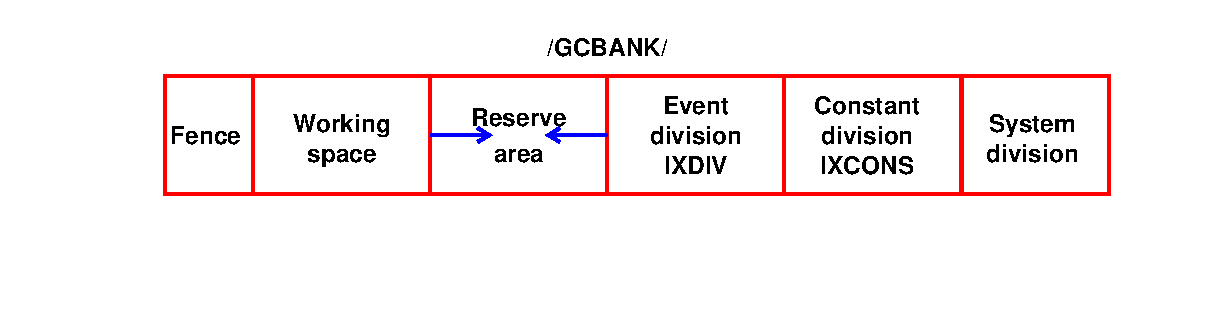
\epsfig{file=eps/base110-1.eps,width=16cm}
      \caption{Layout of the dynamic store}
      \label{fg:base110-1}
\end{figure}

\Shubr{GDINIT}{}
This routine
initialises the {\tt GEANT} drawing package {\tt[DRAW001]} and it has
to be called before any other graphic routine. {\tt GEANT} uses the
CERN-developed {\tt HIGZ}~\cite{bib-HIGZ} graphic library, and this
has to be initialised before the call to \Rind{GDINIT}.
In the example given
in {\tt [BASE100]} the routines \Rind{IGINIT} and \Rind{IGMETA}
are used. Alternatively, the routine \Rind{HPLINT} from HPLOT~\cite{bib-HPLOT}
can be used. This routine calls the appropriate procedures from {\tt HIGZ} to 
initialise the underlaying graphics system. At the moment {\tt HIGZ} can 
use several flavours of GKS~\cite{bib-gks2d,bib-gks3d,bib-GKS1}
and {\tt X11} and it is available on all machines where the CERN Program
Library has been installed.

\Shubr{GPHYSI}{}
Completes the data structure {\tt JMATE}, (see {\tt [PHYS100]}) calculating the
cross-section and stopping power tables.

\Shubr{GBHSTA}{}
Initialises the standard histograms requested by the user via the
data record {\tt HSTA}.
The following histogram keywords may be used :
\begin{DLtt}{MMMMMMMM}
\item[TIME]    time per event;
\item[SIZE]     size of division {\tt IXDIV} per event;
\item[MULT]    total number of tracks per event;
\item[NTRA]    number of {\it long life} tracks per event;
\item[STAK]    maximum stack size per event.
\end{DLtt}

\Rind{GBHSTA} should be called after \Rind{GFFGO}.

\Shubr{GGCLOS}{}
This routine has to be called at the end of the definition
of the geometry by the user, after thal all volumes have been defined
and positioned and all detectors defined. 
Failure to call this routine will prevent
the {\tt GEANT} system from working correctly. Main tasks of this routine
are:
\begin{itemize}
\item close the geometry package;
\item complete the {\tt JVOLUM} data structure;
\item process the detector definition provided by the user;
\item prepare the tables for the tracking speed optimisation requested
by the user via the \Rind{GSORD} routine or the {\tt OPTI} data record.
\end{itemize}
